% lintrans - The linear transformation visualizer
% Copyright (C) 2021-2022 D. Dyson (DoctorDalek1963)

% This program is licensed under GNU GPLv3, available here:
% <https://www.gnu.org/licenses/gpl-3.0.html>

\documentclass[../development.tex]{subfiles}

\begin{document}

\subsubsection{Fixing an animation crash\label{development:fixing-bugs-and-adding-polish:fixing-an-animation-crash}}

The scaling logic in \ref{development:visualizing-matrices:preserving-determinants} creates a matrix $\mathbf{A}$ which is the start matrix plus some proportion of the difference between the target and start matrices. It then defines matrix $\mathbf{B}$ to be the matrix A normalised to have a determinant of 1. We then divide by $\det(\mathbf{B})$ to get matrix $\mathbf{C}$, which we then render.

This works very well for most matrices, but if we're animating from $\mathbf{I}$ to $-\mathbf{I}$ for example, then we can get the following problem:

When we're halfway through the animation, $p = \frac{1}{2}$.
\begin{align*}
\mathbf{A} &= \mathbf{S} + p (\mathbf{T} - \mathbf{S})\\
&= \mathbf{I} + \frac{1}{2} (-\mathbf{I} - \mathbf{I})\\
&= \mathbf{I} + \frac{-1}{\cancel{2}} \cancel{2} \mathbf{I}\\
&= \mathbf{I} - \mathbf{I} = \mathbf{0}
\end{align*}

I'm using $\mathbf{I}$ as an example here, but this can happen with the right $p$ for many matrix pairs. Since $\mathbf{A} = \mathbf{0}$, $\det(\mathbf{A}) = 0$. We check for this case already when we find $c$:

%: f7a91cdc35695f8fb9269b17bc103e42578072bd
%: src/lintrans/gui/main_window.py:367-370 noscopes

But if $\det(\mathbf{A}) = 0$, then $c = 0$ and $\det(\mathbf{B}) = 0$, so we also need to check that before we divide by it.

Old:

%: f7a91cdc35695f8fb9269b17bc103e42578072bd
%: src/lintrans/gui/main_window.py:383-384 noscopes

New:

%: 4383808a4cc29d192c55aca56161d8affda8c9a7
%: src/lintrans/gui/main_window.py:384-391 noscopes

This change fixes a division by zero bug, which eliminates a possible crash here.

\subsubsection{Limiting parallel lines\label{development:fixing-bugs-and-adding-polish:limiting-parallel-lines}}

If you try to render a matrix like \texttt{0.01Irot(45)}, then the app ends up drawing as many parallel lines as it can physically fit in the viewport. This leads to a lot of lag, especially when zoomed out far. To fix this, I just introduced a maximum number of parallel lines. I chose 150 as a number that was big enough to have enough parallel lines for matrices that need a lot, while also causing virtually no lag.

%: bd9aaa2e3037214f65d0fc1d12d67db35af0e5ec
%: src/lintrans/gui/plots/classes.py:169

%: bd9aaa2e3037214f65d0fc1d12d67db35af0e5ec
%: src/lintrans/gui/plots/classes.py:230-277

The idea behind this code is just to limit the maximum number of parallel lines that get drawn. It works perfectly for oblique lines, but there's a small bug for orthogonal lines that I never noticed. I just forgot to test it.

% TODO: Reference the section where I fix this
On lines 234 and 252, I call the built-in \pyinline{max()} function with the maximum number of parallel lines and the total number of lines that could fit in the viewport. This should be a call to \pyinline{min()} instead. I fixed this before releasing it for my end users, but it took an embarrassingly long time to notice something this simple.

\begin{figure}[H]
	\hspace{0.005\linewidth}
	\centering
	\begin{minipage}{0.48\linewidth}
		\centering
		\begin{figure}[H]
			\centering
			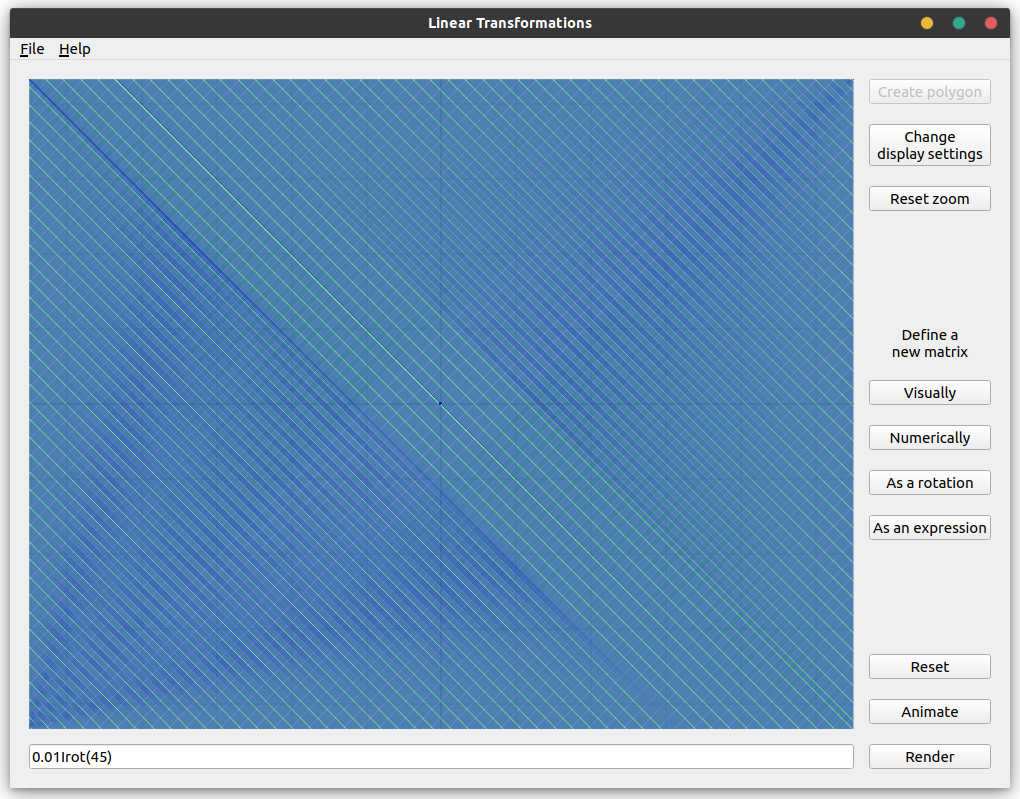
\includegraphics[width=\linewidth]{development/bd9aaa2e3037214f65d0fc1d12d67db35af0e5ec/old.png}
			\caption{The old version with too many parallel lines.}
			\label{fig:development:bd9aaa2e3037214f65d0fc1d12d67db35af0e5ec:old.png}
		\end{figure}
	\end{minipage}%
	\hspace{0.015\linewidth}
	\begin{minipage}{0.48\linewidth}
		\centering
		\begin{figure}[H]
			\centering
			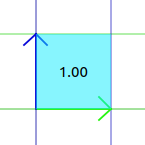
\includegraphics[width=\linewidth]{development/bd9aaa2e3037214f65d0fc1d12d67db35af0e5ec/new.png}
			\caption{The fixed version with a maximum number of parallel lines.}
			\label{fig:development:bd9aaa2e3037214f65d0fc1d12d67db35af0e5ec:new.png}
		\end{figure}
	\end{minipage}
	\hspace{0.005\linewidth}
	\vspace{-1em}
\end{figure}

\end{document}
